\chapter{Results}
\begin{toDo}
	\section{Architecture}
	Mostrare l'architettura del software a livello implementativo
    \section{Pre processing}
    Mostrare i risultati del pre processing.
    \begin{itemize}
        \item serie di Fourier applicate a griglie sintetiche per dedurre quali sono le frequenze di nostro interesse: griglie dritte e ruotate, griglie chiare e scure, griglie con elementi inquinanti, confronto tra teoria e aspettativa
        \item serie di Fourier applicate a immagini vere, confronto con le immagini sintetiche
        \item mostrare alcuni risultati della pulizia dei quadretti attraverso le varie fasi dell'algoritmo di pulizia
    \end{itemize}
    \section{Synthesis}
    Mostrare una piccola analisi delle sintesi ottenute e della velocità del programma, magari con dettagli implementativi
    \section{Comparison}
   		Mostrare dettagli del clustering a livello esecutivo, come velocità del programma e confronto con l'esecuzione su CPU
    	\subsection{Results}
    		Mostrare dettagli in esecuzione dei vari valori ottenuti dall'algoritmo di comparazione. Quindi concludere con una panoramica dei risultati ottenuti.
\end{toDo}


%\begin{figure}
%	\centering
%	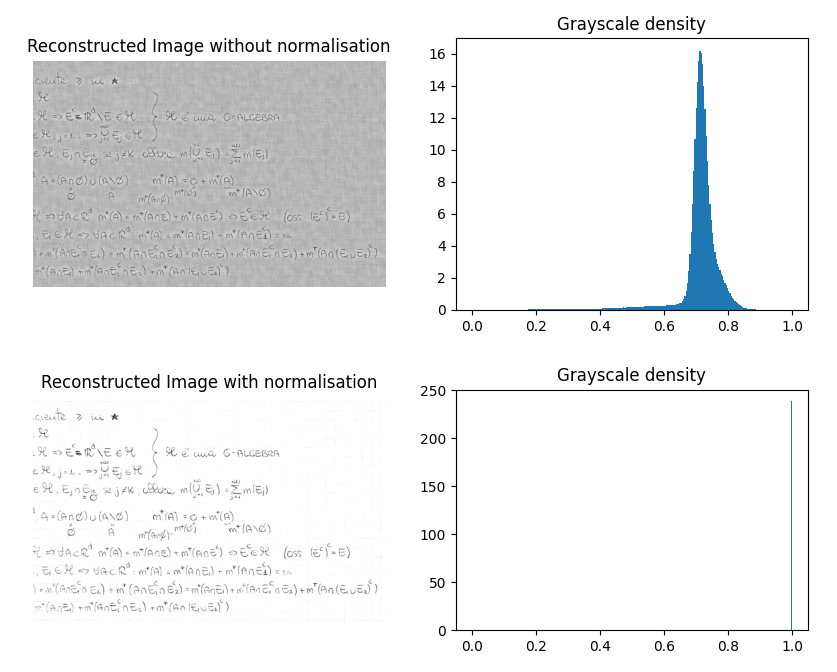
\includegraphics[width=\linewidth]{Figures/first_reconstruct.png}
%	\caption{Come si osserva i grigi si sono molto avvicinati tra loro dopo \gls{fft}, ma è possibile ribilanciare i colori confrontandoli con l'immagine originale.}
%	\label{fig:first_reconstruct}
%\end{figure}
